\chapter{Results}
\label{chap:results}

\section{Experimental Setup}
\subsection{Test Machine}
All measurements were gathered from a single machine with an NVIDIA Tesla K40c and NVIDIA GTX TITAN Black.
The Tesla K40c and GTX TITAN Black are two of NVIDIA's higher end solutions.
The GTX TITAN Black, which we'll now refer to as Black, has a 0.98 GHz GPU clock rate, 3.5 GHz memory clock rate, and 6 GB of memory.
The Tesla K40c, now K40c, has a 0.88 GHz GPU clock rate, 3.0 GHz memory clock rate, and 12 GB of memory.
The Black is faster than the K40c, but has significantly less memory.
Both the CUDA runtime and driver version were 6.0.
The binary was compiled using -O3 optimization and compute capability 2.0.
We chose the more compatible compute capability 2.0 instead of 3.5, because we did not need any of the features of 3.5.
Timings were recorded using the CUDA events API.

\subsection{Data}

Data for our evaluation was gathered from various publicly available datasets, often used in benchmarking lossless compression algorithms.

\section{Suffix Array}

\begin{figure}[ht!]
\centering
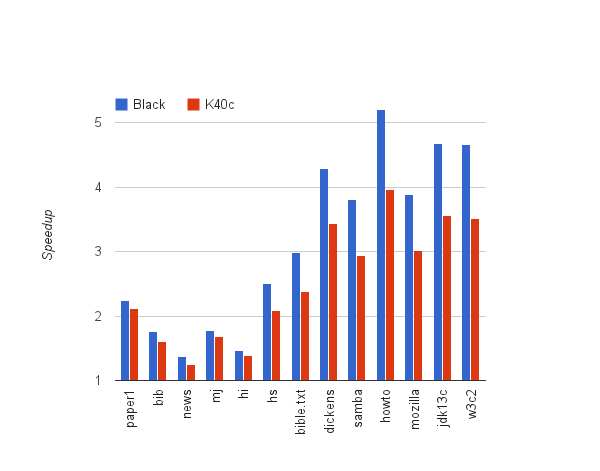
\includegraphics[width=1.0\textwidth]{images/saresult.png}
\caption{Speedup of suffix array construction on the GPU compared to the fastest CPU implementation}
\label{fig:saresult}
\end{figure}

\begin{table}[h]
\begin{tabular}{@{}lllllll@{}}
\toprule
size(MB) & filename  & Black(ms)  & K40c(ms)   & CPU(ms)   & Black Speedup & Black ms/B \\ \midrule
0.05     & paper1    & 15.2   & 16     & 34    & 2.2           & 0.286          \\
0.11     & bib       & 19.3   & 21.2   & 34    & 1.8           & 0.173          \\
0.36     & news      & 33.6   & 36.8   & 46    & 1.4           & 0.089          \\
0.43     & mj        & 29.2   & 30.9   & 52    & 1.8           & 0.065          \\
0.49     & hi        & 34.2   & 36.1   & 50    & 1.5           & 0.067          \\
3.14     & hs        & 108.5  & 130.6  & 272   & 2.5           & 0.033          \\
3.86     & bible.txt & 112.9  & 141.5  & 338   & 3.0           & 0.028          \\
9.72     & dickens   & 282.8  & 353.5  & 1212  & 4.3           & 0.028          \\
20.61    & samba     & 536.9  & 693    & 2042  & 3.8           & 0.025          \\
37.60    & howto     & 1021.1 & 1339.7 & 5320  & 5.2           & 0.026          \\
48.85    & mozilla   & 1278.2 & 1642.6 & 4958  & 3.9           & 0.025          \\
66.50    & jdk13c    & 1928.2 & 2525.4 & 9010  & 4.7           & 0.028          \\
99.37    & w3c2      & 2896   & 3840.8 & 13486 & 4.7           & 0.028          \\ \bottomrule
\end{tabular}
\caption{Runtimes(ms), speedups, and ms/B of datasets for evaluation of suffix array construction}
\label{tab:sadata}
\end{table}

The evaluation of the suffix array is actually an evaluation of a reimplementation of the fastest known GPU suffix array construction algorithm (SACA) by Deo and Keely \cite{Deo}.
The benefits and applications of the suffix array has already been detailed in Section~\ref{sec:sa} 
Deo and Keely's evaluation was done on an AMD Radeon GPU using OpenCL.
Our results on a NVIDIA GPU using CUDA and CUB primitives with ModernGPU's merge path method to mergesort are not expected to be significantly different.
We will be comparing our results to a set of SACA benchmarks found on the wiki of LibDivSufSort, one of if not the fastest CPU SACA implementation \cite{SACA}.
That benchmark compares the fastest CPU SACA implementations on a variety of test files.
We will compare our GPU implementation against the fastest CPU time for each file.
Files were picked to match closely with Deo and Keely's evaluation.
GPU times include parsing the file, transferring the data both ways, and the construction of the suffix array.

Figure~\ref{fig:saresult} and Table~\ref{tab:sadata} presents the results comparing the CPU implementations to our GPU implementation.
The first thing to note is that the CPU SACA benchmarks are significantly faster than those used by Deo and Keely.
Our GPU implementation did not see the speedup of 35x that theirs did, but we still found around a 4-5x speedup for most files for Black.
We did not have their implementation or their raw result data to compare against.
Loosely comparing with the charts in their paper though, we find that our GPU implementation is at least on par if not faster.

Another interesting metric is the runtime in microseconds per Byte seen in \cite{al2012comparison}.
We found that after a certain point, our Black implementation was achieving rates of around 0.02 to 0.03 ms/B.
In comparison, \cite{al2012comparison} found results between 0.1 to 0.4 ms/B.

Like many other GPU algorithms, we found that smaller files did not see the greater speedups that larger files did.
The likely cause is that smaller files cannot fully saturate the GPU, and the cost of initialization and data transfer could not be hidden by increased computations.
This indicates that the GPU is not the all around solution for faster suffix arrays and the size of the input needs to be considered.

\begin{figure}[ht!]
\centering
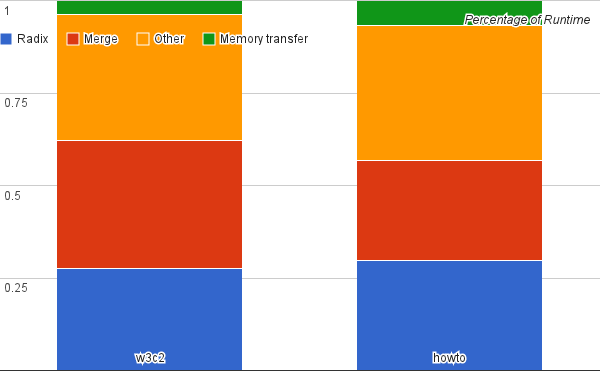
\includegraphics[width=1.0\textwidth]{images/saprofile.png}
\caption{Profile of Suffix Array construction on the GPU}
\label{fig:saprofile}
\end{figure}

Figure~\ref{fig:saprofile} shows a profile of the SACA of the GPU implementation.
Kernels other than those involved in the merging or sorting take the greatest percentage of time in both examples.
These kernels have the most room for improvement, since they are less likely to deal with primitives and more likely deal with the setup and movement of data.
The CUDA grid and block sizes could have a greater factor in the speeds and further optimization are more likely to see gains here.

%aug 24 2008

\section{ANSV}

\begin{figure}[ht!]
\centering
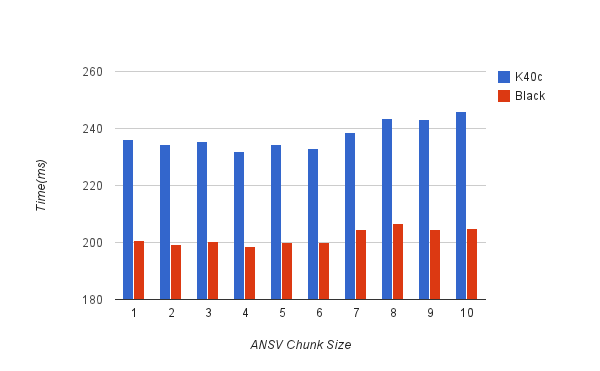
\includegraphics[width=1.0\textwidth]{images/ansvsize.png}
\caption{The effect of chunk size on ANSV runtime on the GPU}
\label{fig:ansvresult}
\end{figure}

he ANSV algorithm divides the suffix array into chunks for each thread.
These threads will then individually solve the ANSV problem on their chunk and solve any outliers using a preconstructed binary tree.

Figure~\ref{fig:ansvresult} shows the impact of changing the chunk size in the ANSV generation.
For our setup we can see a noticeable speedup at a chunk size of 4.
The chunk size of 4 is not a universal speedup for all NVIDIA GPUs.
Although not presented in this paper, a mobile GPU, NVIDIA GT 650M, found speedups at a much greater chunk size.
Different hardware have different memory latencies and other costs.

%Figure~\ref{fig:ansvresult} shows a profile of the ANSV generation in the two main steps, the construction of the binary tree and the chunk processing with a chunk size of 4. 
%The construction of the min tree was no more than 4 percent of the overall ANSV generation.
%Several future optimizations were discussed earlier for the min tree, but seeing as it is only a small percentage of the overall runtime, time is probably better spent somewhere else.
%See Amdahl's law \cite{amdahl1967validity}.
%The bigger chunk of the runtime is in the chunk processing, as expected.

\section{PLZ}
\begin{figure}[ht!]
\centering
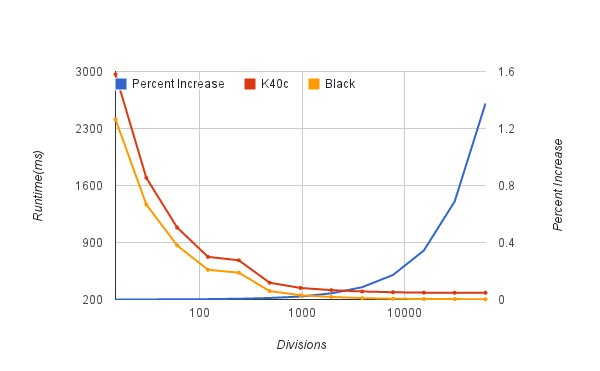
\includegraphics[width=1.0\textwidth]{images/lzchart.png}
\caption{The effects of chunk size on percent increase and runtimes}
\label{fig:lzchart}
\end{figure}

% Please add the following required packages to your document preamble:
% \usepackage{booktabs}
\begin{sidewaystable}[h]
\begin{tabular}{@{}|l|l|l|l|l|l|l|l|l|l|l|l|l|@{}}
\toprule
filename         & \begin{tabular}[c]{@{}l@{}}filesize\\ (MB)\end{tabular} & Black & K40c & lz-og & lz-ansv & plz3 & \begin{tabular}[c]{@{}l@{}}lz-og\\ Speedup\\ Black\end{tabular} & \begin{tabular}[c]{@{}l@{}}lz-ansv\\ Speedup\\ Black\end{tabular} & \begin{tabular}[c]{@{}l@{}}plz3\\ Speedup\\ Black\end{tabular} & LZ      & PLZ     & \begin{tabular}[c]{@{}l@{}}percent\\ increase\end{tabular} \\ \midrule
10Mrandom    & 9.5                                                     & 0.3   & 0.4  & 4.7   & 4.0     & 0.4  & 15.85                                                           & 13.47                                                             & 1.48                                                           & 1426311 & 1426496 & 0.013                                                      \\
chr22.dna    & 33.0                                                    & 1.1   & 1.4  & 22.0  & 19.4    & 1.6  & 20.73                                                           & 18.28                                                             & 1.48                                                           & 2461478 & 2461728 & 0.010                                                      \\
howto.txt    & 37.6                                                    & 1.3   & 1.6  & 25.5  & 24.0    & 1.8  & 20.03                                                           & 18.85                                                             & 1.43                                                           & 3063929 & 3064227 & 0.010                                                      \\
jdk13c       & 66.5                                                    & 2.3   & 2.9  & 41.4  & 40.4    & 2.9  & 18.10                                                           & 17.66                                                             & 1.25                                                           & 1209676 & 1210015 & 0.028                                                      \\
wikisamp.xml & 95.4                                                    & 3.4   & 4.3  & 61.4  & 59.9    & 4.0  & 18.21                                                           & 17.76                                                             & 1.20                                                           & 2888810 & 2889040 & 0.008                                                      \\
w3c2         & 99.4                                                    & 3.9   & 5.0  & 84.1  & 63.1    & 4.4  & 21.55                                                           & 16.17                                                             & 1.13                                                           & 2340638 & 2341016 & 0.016                                                      \\
etext99      & 100.4                                                   & 4.0   & 5.2  & 75.2  & 69.9    & 4.8  & 18.97                                                           & 17.63                                                             & 1.21                                                           & 8306413 & 8306658 & 0.003                                                      \\
sprot34.dat  & 104.5                                                   & 4.1   & 5.2  & 72.2  & 69.0    & 4.6  & 17.69                                                           & 16.90                                                             & 1.13                                                           & 6395921 & 6396224 & 0.005                                                      \\
rctail96     & 109.4                                                   & 4.1   & 5.2  & 96.5  & 70.0    & 4.8  & 23.54                                                           & 17.07                                                             & 1.16                                                           & 3905843 & 3906149 & 0.008                                                      \\
rfc          & 111.0                                                   & 4.3   & 5.5  & 76.6  & 72.8    & 4.8  & 17.81                                                           & 16.93                                                             & 1.12                                                           & 5656068 & 5656367 & 0.005                                                      \\ \bottomrule
\end{tabular}
\caption{Sizes, running times(seconds), and speedups of datasets for evaluation of LZ factorization. GPU implementations use PLZ with 480 divisions}
\label{tab:lzdata}
\end{sidewaystable}

To directly compare the generation of PLZ to algorithms and implementations generating the ideal LZ factorization would be unfair.
The outputs are totally different, as the PLZ has lost an important property of the ideal LZ factorization, the LPF.
The LPF in the PLZ are no longer the longest, as discussed in our implementation.
What can be done is a relative comparison to previous implementations.
We will present the percent increase of the PLZ from the LZ factorization to help in the evaluation.

The data set and CPU benchmarks will be taken directly from the results in \cite{shun2013practical}. 
Specifically, we will compare our results to their benchmarks of LZ-OG, the most time efficient single threaded algorithm as seen in \cite{ohlebusch2011lempel}, LZ-ANSV, the sequential algorithm which computes the LZ factorization without every LPF value using lazy LZ factorization, and their contribution PLZ3, their parallel CPU algorithm using 40 cores with hyper-threading.
LZ-ANSV is the closest sequential algorithm after the ANSV generation, while the ANSV generation algorithm comes from PLZ3.

The first and most important metric to look at is how the PLZ chunk size affects the final LZ factorization size.
If the percent increase is too great, then the usage of PLZ is unacceptable.
What percent increase is too great is a judgement that must be made by each user, as each user will have their own requirements.
To pick the different chunk sizes, we decided to use number of divisions as the parameter, although we could have used the actual block size as mentioned before.
More specifically we used multiples of the number of SMs (15).
To try and get a wide range, we used powers of 2 to multiply.

The second most important metric is how the chunk sizes affect the runtimes. 
Since the suffix array construction and the ANSV generation are unrelated, we will keep our focus on the LPF time.
This time assumes the suffix array and ANSV arrays are already present on GPU memory.
It includes the generation of the necessary LPF and PrevOcc arrays, the isolation of the needed values using CUB's deviceSelect, and the data copy of those values back to the CPU.
Many LZ factorization papers evaluate the runtime of their algorithm starting after the suffix array is in memory.
We will consider that runtime later.

Figure~\ref{fig:lzchart} presents the results with these two metrics together.
We show the effect of percent increase and runtime as a function of the number of divisions.
First, we notice that the percent increase grows linearly with the number of divisions.
This trend is intuitive as each extra division has a chance to increase the final PLZ length if the division boundary occurs between the ideal LZ factorization.
Next, we notice that the runtime generally decreases rapidly as we increase the number of divisions.
At some point however, the rapid decreases stops and increasing the divisions further does not have as much effect on the runtime.
As we can see in Figure~\ref{fig:lzchart}, this occurs at around 480 divisions for both cards.
At 480 divisions the datasets have 0.01 average percent increase.
For some perspective, a file that compresses to 1 MB using the ideal LZ factorization would require an additional 105 bytes using PLZ.
At this point, the Black has an average runtime of 303.7 ms, while the K40c has an average runtime of 406.8 ms.
As we increase the number of divisions from 480 to 30720, Black's runtime decreases only 30 percent, while the percent increase changes over 150 percent to 1.54 percent.
Similarly, K40c's runtime decreases only 32 percent.
We will use this 0.01 percent increase with 480 divisions for the rest of this evaluation.

We now take a look at how our GPU implementation compares to the CPU LZ factorization implementations mentioned earlier.
Table~\ref{tab:lzdata} tabulates the results and speedups found in our experiments.
Our GPU implementation outperforms LZ-OG and LZ-ANSV on all the data sets.
Black sees speedups between 15-24x (19.25x average) compared to LZ-OG and speedups between 13-19x (17.07x average) compared to LZ-ANSV.
When compared to the 40 core PLZ3 implementation, Black performs comparatively with speedups of 1.1-1.5x (1.26x average).
The slower, K40c sees speedups of 12-19x (15.02x) and 10-15x (13.32x) against LZ-OG and LZ-ANSV respectively.
K40c performed comparatively with PLZ3 having speedups and slowdowns no greater than 1.2x (0.98x average).

\begin{figure}[ht!]
\centering
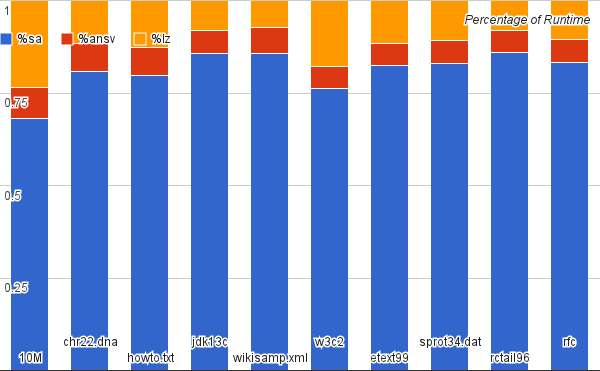
\includegraphics[width=1.0\textwidth]{images/allprof.png}
\caption{Profile of GPU implementation}
\label{fig:allprof}
\end{figure}

Figure~\ref{fig:allprof} shows a profile of the three main sections of our implementation, the SA, the ANSV, and the LZ.
The majority of our implementation, like most LZ factorization implementations, spend most of their time constructing the suffix array.
The suffix array construction takes on average 81 percent of the overall time.

Highly compressible inputs are excluded from the above results.
These files incur an incredible space cost when using PLZ, as each division is likely to add an additional factor to the factorization.
An additional factor with a highly compressible input could and probably will result in very high percent increases.
Specifically, the file 10Midentical contained only one character.
The resulting ideal LZ factorization contained 2 factors.
Each PLZ division increased the LZ factorization by 1 factor.
With 480 divisions, we found 481 factors with the PLZ LZ factorization, amounting to an increase of 23950 percent.
